\documentclass[12pt,a4paper]{article}
\newcommand{\reportTitle}{Laboratory work 5:}
\newcommand{\reportSubject}{Study and Empirical Analysis of\\[0.3cm]Prim and Kruskal Greedy Algorithms}
\usepackage{iftex}
\ifPDFTeX
    \usepackage[T1]{fontenc}
    \usepackage[utf8]{inputenc}
    \usepackage{mathptmx}
    \usepackage{courier}
\else
    \usepackage{fontspec}
    \setmainfont{Times New Roman}
    \setmonofont{Courier New}
\fi

\usepackage{amsmath}
\usepackage{graphicx}
\usepackage{float}
\usepackage[english]{babel}
\usepackage{indentfirst}
\usepackage{geometry}
\geometry{
    a4paper,
    left=20mm,
    right=10mm,
    top=20mm,
    bottom=20mm
}

\usepackage{setspace}
\setstretch{1.5}
\setlength{\parindent}{1.25cm}
\setlength{\parskip}{0pt}

\usepackage{titlesec}
\titleformat{\section}
  {\normalfont\bfseries\centering\fontsize{13}{15}\selectfont\MakeUppercase}{\thesection}{0.8em}{}
\titleformat{\subsection}
  {\normalfont\bfseries\fontsize{12}{14}\selectfont}{\thesubsection}{0.8em}{}
\titleformat{\subsubsection}
  {\normalfont\bfseries\fontsize{12}{14}\selectfont}{\thesubsubsection}{0.8em}{}

\titlespacing*{\section}{0pt}{0pt}{0.8\baselineskip}
\titlespacing*{\subsection}{0pt}{0.6\baselineskip}{0.3\baselineskip}
\titlespacing*{\subsubsection}{0pt}{0.4\baselineskip}{0.2\baselineskip}

\setcounter{secnumdepth}{3}

\usepackage{booktabs}
\usepackage{array}
\usepackage{longtable}
\usepackage{chngcntr}
\usepackage{caption}
\usepackage{subcaption}
\usepackage{enumitem}
\usepackage{needspace}
\usepackage{xcolor}
\usepackage{listings}
\usepackage{tocloft}

\setlist[itemize]{label=--,leftmargin=1.25cm,itemsep=0pt,topsep=0pt}
\setlist[enumerate]{leftmargin=1.25cm,itemsep=0pt,topsep=0pt}

\renewcommand{\cftsecleader}{\cftdotfill{1}}
\renewcommand{\cftsubsecleader}{\cftdotfill{1}}
\renewcommand{\cftsubsubsecleader}{\cftdotfill{1}}
\setlength{\cftbeforesecskip}{0pt}
\setlength{\cftbeforesubsecskip}{0pt}
\setlength{\cftbeforesubsubsecskip}{0pt}
\setlength{\cftsecindent}{0pt}
\setlength{\cftsubsecindent}{0.5cm}
\setlength{\cftsubsubsecindent}{1cm}
\setlength{\cftsecnumwidth}{1.0cm}
\setlength{\cftsubsecnumwidth}{1.0cm}
\setlength{\cftsubsubsecnumwidth}{1.2cm}
\renewcommand{\cftsecfont}{\bfseries}
\renewcommand{\cftsubsecfont}{\normalfont}
\renewcommand{\cftsecpagefont}{\bfseries}
\renewcommand{\cftsubsecpagefont}{\normalfont}
\renewcommand{\cfttoctitlefont}{\hfill\normalfont\Large\bfseries}
\renewcommand{\cftaftertoctitle}{\hfill}
\setcounter{tocdepth}{2}

\usepackage{hyperref}
\usepackage{bookmark}
\hypersetup{
    hidelinks,
    linktoc=all
}
\addto\captionsenglish{\renewcommand{\contentsname}{TABLE OF CONTENTS}}
\renewcommand{\contentsname}{TABLE OF CONTENTS}

\counterwithin{figure}{section}
\counterwithin{table}{section}
\counterwithin{equation}{section}

\newcommand{\reportcodestyle}{\linespread{1}\ttfamily\fontsize{10}{10}\selectfont}

\lstset{
    basicstyle=\reportcodestyle,
    frame=none,
    breaklines=true,
    columns=fullflexible,
    keepspaces=true,
    showstringspaces=false,
    aboveskip=0.2\baselineskip,
    belowskip=0.2\baselineskip
}

\captionsetup[figure]{
    font=bf,
    labelfont=bf,
    textfont=bf,
    labelsep=endash,
    justification=centering,
    singlelinecheck=false
}
\captionsetup[table]{
    font=normalfont,
    labelfont=normalfont,
    textfont=normalfont,
    labelsep=endash,
    justification=raggedleft,
    singlelinecheck=false,
    position=above
}

\newcommand{\studentName}{Ple\c{s}u Dinu}
\newcommand{\studentGroup}{FAF-241}
\newcommand{\teacherTitle}{asist. univ.}
\newcommand{\teacherName}{Fi\c{s}tic Cristofor}
\newcommand{\reportYear}{2026}
\newcommand{\reportCity}{Chi\c{s}in\u{a}u}

\newcommand{\makelabtitle}{
    \begin{titlepage}
        \centering

        \textbf{\large Ministerul Educa\c{t}iei \c{s}i Cercet\u{a}rii al Republicii Moldova}\\[0.3cm]
        \textbf{\large Universitatea Tehnic\u{a} a Moldovei}\\[0.3cm]
        \textbf{\large Facultatea Calculatoare, Informatic\u{a} \c{s}i Microelectronic\u{a}}\\[3cm]

        \vfill

        {\LARGE \reportTitle}\\[0.5cm]
        {\LARGE \reportSubject}\\[3cm]

        \vfill

        \begin{flushleft}
            \hspace{1cm}
            \begin{minipage}{0.8\textwidth}
                {\large Elaborated:}\\
                {\large st.\ gr.\ \studentGroup \hfill \studentName}\\[0.8cm]
                {\large Verified:}\\
                {\large \teacherTitle \hfill \teacherName}\\
            \end{minipage}
        \end{flushleft}

        \vfill

        {\large \reportCity\ - \reportYear}
    \end{titlepage}
}

\newcommand{\startreport}{
    \begin{document}
    \makelabtitle
    \newpage
    \pagenumbering{arabic}
    \setcounter{page}{2}
    \thispagestyle{empty}
    \tableofcontents
    \thispagestyle{empty}
    \newpage
}

\newcommand{\reportprelimsection}[1]{
    \newpage
    \section*{#1}
    \thispagestyle{empty}
    \phantomsection
    \addcontentsline{toc}{section}{#1}
}

\newcommand{\reportintroduction}{
    \newpage
    \section*{INTRODUCTION}
    \phantomsection
    \addcontentsline{toc}{section}{INTRODUCTION}
}

\newcommand{\reportmainsection}[1]{
    \newpage
    \section{#1}
}

\newcommand{\tocsubsection}[1]{
    \Needspace{12\baselineskip}
    \subsection{#1}
}

\newcommand{\reportlabel}[1]{
    \Needspace{6\baselineskip}
    \par\noindent\textbf{#1}\par
}

\newcommand{\reportfrontsubsection}[1]{
    \subsection*{#1}
    \phantomsection
    \addcontentsline{toc}{subsection}{#1}
}

\newcommand{\reportunnumberedsection}[1]{
    \newpage
    \section*{#1}
    \phantomsection
    \addcontentsline{toc}{section}{#1}
}

\newcommand{\reportreferences}[1]{
    \newpage
    \section*{REFERENCES}
    \phantomsection
    \addcontentsline{toc}{section}{REFERENCES}
    \begin{thebibliography}{99}
    #1
    \end{thebibliography}
}


\startreport


\reportintroduction
A minimum spanning tree of a connected weighted undirected graph is a subgraph that connects all vertices using exactly \(|V| - 1\) edges such that the total edge weight is minimized. Minimum spanning trees arise naturally in a wide range of practical problems: designing minimum-cost telecommunication or electrical networks, constructing road or pipeline infrastructure that connects all sites with the least total length, clustering data points by removing the heaviest edges from the spanning tree, and approximating solutions to the Travelling Salesman Problem. The MST of a graph is not necessarily unique, but its total weight is always the same regardless of which specific MST is selected.

Two classical algorithms for constructing minimum spanning trees are studied in this laboratory. Prim's algorithm grows the spanning tree vertex by vertex starting from an arbitrary source. At each step the cheapest edge connecting a vertex already in the tree to a vertex not yet included is added, until all vertices belong to the tree. Kruskal's algorithm takes a global view: it sorts all edges in non-decreasing order of weight and adds each edge to the forest if and only if it does not create a cycle, continuing until \(|V| - 1\) edges have been selected.

Both algorithms are guaranteed to produce a minimum spanning tree on any connected weighted undirected graph, but they do so through fundamentally different strategies. Prim resembles Dijkstra's algorithm in structure and is well-suited to dense graphs where many edges are available at each step. Kruskal is better suited to sparse graphs where sorting the edges is cheap relative to the total work. In practice, the choice between them depends on the graph structure and the quality of the available data structures.

The efficiency of both algorithms depends critically on the internal data structures used. For Prim, the bottleneck is the selection of the next cheapest edge; using a priority queue instead of a linear scan reduces this from \(O(V^2)\) to \(O(E \log V)\) total. For Kruskal, the bottleneck is the cycle-detection step; using a union-find data structure with path compression and union by rank reduces this to nearly \(O(E \alpha(V))\) amortized, where \(\alpha\) is the inverse Ackermann function, which is effectively constant for all practical graph sizes.

Classic and optimized variants of both algorithms were tested on connected weighted undirected graphs at several sizes and density levels. The aim was to see how much the optimized data structures actually help in practice and whether the choice between Prim and Kruskal matters more than density level.

\reportmainsection{ALGORITHM ANALYSIS}

\tocsubsection{Objective}
Study and analyze Prim and Kruskal on connected weighted undirected graphs with increasing size and different density.

\tocsubsection{Tasks}
\begin{enumerate}[leftmargin=1.25cm]
    \item study the greedy algorithm design technique;
    \item implement Prim and Kruskal in a programming language;
    \item perform empirical analysis of the two algorithms;
    \item increase the number of nodes in the graph and analyze the influence on the algorithms;
    \item make a graphical presentation of the obtained data;
    \item formulate conclusions.
\end{enumerate}

\tocsubsection{Theoretical Notes}
Greedy algorithms build a solution incrementally by always making the locally optimal choice at each step, without reconsidering earlier decisions. For a greedy strategy to yield a globally optimal solution, the problem must exhibit the greedy-choice property: a global optimum can always be reached by including the locally best choice made at the current step. The minimum spanning tree problem possesses this property, which can be formalized through matroid theory. The graph matroid structure guarantees that any greedy algorithm that always selects the minimum-weight edge not forming a cycle will produce a minimum spanning tree \cite{gfg-greedy,tp-greedy}.

The correctness of MST algorithms rests on two fundamental properties of minimum spanning trees. The cut property states that for any cut of the graph (a partition of vertices into two non-empty sets), the minimum-weight edge crossing the cut belongs to some minimum spanning tree. Prim exploits this property directly: at each step the growing tree forms one side of a cut, and the cheapest crossing edge is added. The cycle property states that for any cycle in the graph, the maximum-weight edge of that cycle does not belong to any minimum spanning tree (assuming unique edge weights). Kruskal exploits this property: it never adds an edge that closes a cycle, so the heaviest edge in any cycle is always excluded.

Prim's algorithm in its classic form maintains a key array recording the minimum-weight edge from each vertex to the current tree. At each of the \(V\) steps, the algorithm scans all unselected vertices to find the one with the smallest key, costing \(O(V)\) per step and \(O(V^2)\) in total. For each newly added vertex, the key values of its neighbors are updated if a cheaper connection is found, adding \(O(E)\) total update work. The overall classic complexity is therefore \(O(V^2 + E) = O(V^2)\). The optimized variant stores unselected vertices in a binary min-heap keyed by their current minimum edge weight. Each extraction costs \(O(\log V)\) and each key update (decrease-key) costs \(O(\log V)\), giving \(O(V \log V)\) for all extractions and \(O(E \log V)\) for all updates, for an overall complexity of \(O(E \log V)\). On dense graphs with \(E = O(V^2)\), the classic \(O(V^2)\) can be faster than the optimized \(O(V^2 \log V)\) due to lower constant factors \cite{scaler}.

Kruskal's algorithm first sorts all \(|E|\) edges by weight, costing \(O(E \log E)\). It then processes each edge in sorted order and checks whether its two endpoints belong to different components of the current forest. The classic implementation represents each component as a set of vertices; the component membership test requires a linear scan taking \(O(V)\) in the worst case, giving \(O(V \cdot E)\) for all tests. The optimized implementation uses a union-find data structure with path compression and union by rank. The \texttt{find} operation with path compression identifies the component root in nearly \(O(1)\) amortized time, and the \texttt{union} operation merges two components in \(O(\alpha(V))\) amortized time, where \(\alpha\) is the inverse Ackermann function. The total complexity is therefore \(O(E \log E + E \cdot \alpha(V)) = O(E \log E)\) dominated by the sorting step.

The practical choice between Prim and Kruskal depends on graph density. On dense graphs where \(E = O(V^2)\), the edge list for Kruskal contains \(O(V^2)\) elements and sorting costs \(O(V^2 \log V)\), while Prim's classic variant costs only \(O(V^2)\). Dense graphs therefore favor Prim. On sparse graphs where \(E = O(V)\), Kruskal's sorting costs \(O(V \log V)\) and its union-find operations cost nearly \(O(V)\), while Prim's heap variant costs \(O(E \log V) = O(V \log V)\) — the two are comparable, but Kruskal often wins due to its simpler access pattern and better cache locality when processing a sorted edge array sequentially.

\tocsubsection{Comparison Metric}
Four values were recorded for each run:
\begin{itemize}[leftmargin=1.25cm]
    \item execution time in milliseconds;
    \item peak memory usage in kilobytes;
    \item total weight of the minimum spanning tree;
    \item number of edges and graph density.
\end{itemize}

\tocsubsection{Input Format}
The benchmark used connected weighted undirected graphs with random edge weights from 1 to 20. Three graph categories were generated:
\begin{itemize}[leftmargin=1.25cm]
    \item sparse graphs;
    \item medium-density graphs;
    \item dense graphs.
\end{itemize}

The tested graph sizes were 100, 200, 350, 500, and 700 vertices.

\reportmainsection{IMPLEMENTATION}

\tocsubsection{Prim}
Two Prim variants were implemented. The classic version selects the next vertex by scanning all candidates linearly; the optimized one uses a priority queue instead, bringing the per-step cost down from \(O(V)\) to \(O(\log V)\) \cite{repo}.

\subsubsection{Algorithm Description}

The method follows the idea shown in the next pseudocode.

\begin{lstlisting}
Prim(graph, start):
    mark start as part of the tree
    push all outgoing edges of start in priority queue
    while the queue is not empty:
        extract the cheapest edge
        if it reaches an unvisited vertex:
            add that edge to the tree
            add outgoing edges of the new vertex to the queue
    return minimum spanning tree
\end{lstlisting}

\subsubsection{Implementation}

The heap brings a clear speed advantage, but every newly added vertex pushes its neighbors into the queue, so dense graphs drive memory usage up considerably.

\begin{lstlisting}
# Classic -- O(V^2) linear minimum selection over adjacency matrix
def prim_classic(graph, start=0):
    n = graph.num_vertices
    matrix = graph.to_matrix()
    selected = [False] * n
    min_edge = [float("inf")] * n
    min_edge[start] = 0
    total_weight = 0
    for _ in range(n):
        v = min((i for i in range(n) if not selected[i]),
                key=lambda i: min_edge[i])
        selected[v] = True
        total_weight += min_edge[v]
        for u in range(n):
            w = matrix[v][u]
            if w and not selected[u] and w < min_edge[u]:
                min_edge[u] = w
    return total_weight

# Optimized -- O(E log V) heap-based priority queue
def prim_optimized(graph, start=0):
    visited = set()
    heap = [(0, start)]
    total_weight = 0
    while heap and len(visited) < graph.num_vertices:
        weight, vertex = heapq.heappop(heap)
        if vertex in visited:
            continue
        visited.add(vertex)
        total_weight += weight
        for neighbor, edge_weight in graph.adj[vertex]:
            if neighbor not in visited:
                heapq.heappush(heap, (edge_weight, neighbor))
    return total_weight
\end{lstlisting}

\subsubsection{Results}

Table~\ref{tab:lab5-dense} shows the results at the largest dense graph (700 nodes).

\begin{table}[H]
    \caption{MST benchmark on dense graphs at 700 nodes}
    \label{tab:lab5-dense}
    \centering
    {\fontsize{11}{11}\selectfont\renewcommand{\arraystretch}{1}\begin{tabular}{lllll}
\toprule
Algorithm & Time (ms) & Memory (KB) & MST weight & Edges \\
\midrule
Kruskal\_Classic & 589.288 & 1582.46 & 699 & 122760.0 \\
Kruskal\_Optimized & 545.990 & 1440.25 & 699 & 122760.0 \\
Prim\_Classic & 1330.551 & 3879.47 & 699 & 122760.0 \\
Prim\_Optimized & 435.591 & 7302.00 & 699 & 122760.0 \\
\bottomrule
\end{tabular}
}
\end{table}

The optimized Prim variant was fastest at \(435.6\) ms, but also consumed the most memory --- the time-space trade-off of the heap is directly visible in the data. Figure~\ref{fig:lab5-main} shows overall performance across all sizes.

\begin{figure}[H]
    \centering
    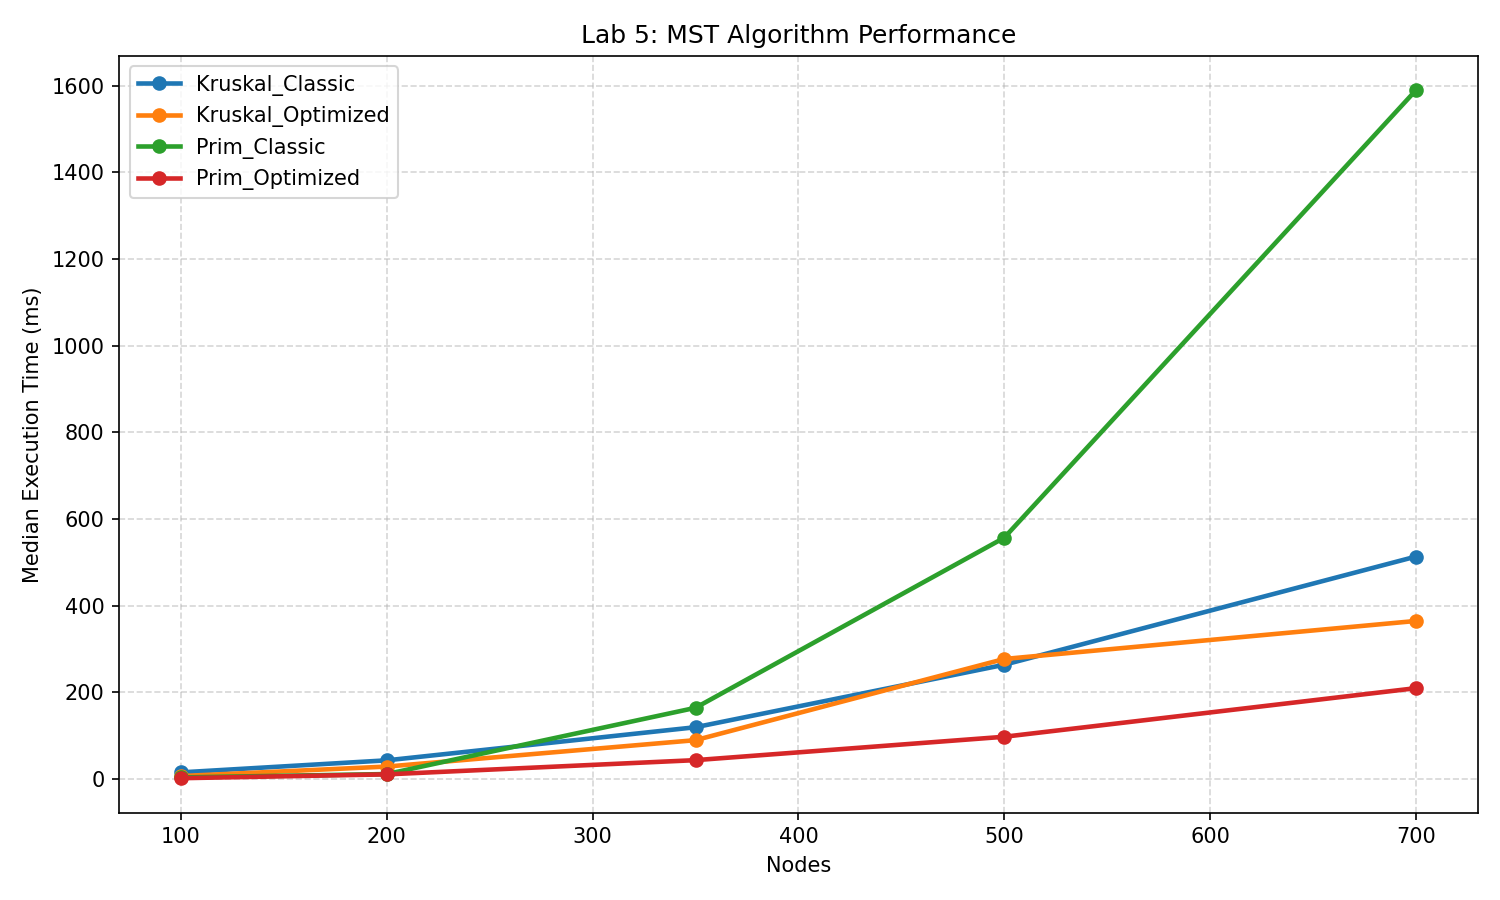
\includegraphics[width=0.88\textwidth]{../../Lab5/plots/mst_performance.png}
    \caption{Overall MST performance}
    \label{fig:lab5-main}
\end{figure}

The growth is especially pronounced for classic Prim, which struggles even on moderately sized graphs.

\subsubsection{Conclusion}

Prim is effective for minimum spanning tree construction, but its practical performance depends heavily on the data structure used for edge selection. At 700 nodes on dense graphs the optimized variant required \(435.6\) ms while the classic required \(1330.6\) ms, a speedup of approximately \(3.1\times\). On sparse graphs the advantage was even larger: the optimized variant required only \(126.3\) ms while the classic required \(1318.2\) ms, a speedup of approximately \(10.4\times\), because the heap contains far fewer candidate edges on sparse graphs and each extraction is correspondingly cheaper. The trade-off is memory: on the 700-node dense graph the optimized variant consumed \(7302\) KB due to heap allocation, while the classic required only \(3879\) KB.

\tocsubsection{Kruskal}
Two Kruskal variants were also implemented. The classic one detects cycles by scanning component sets linearly; the optimized one uses union-find with path compression and rank, making each check nearly constant-time.

\subsubsection{Algorithm Description}

The Kruskal method follows the idea shown in the next pseudocode.

\begin{lstlisting}
Kruskal(graph):
    sort all edges increasingly by weight
    make one component for each vertex
    for each edge in sorted order:
        if the two endpoints are in different components:
            add edge to the tree
            merge the two components
    return minimum spanning tree
\end{lstlisting}

\subsubsection{Implementation}

The union-find structure is compact --- two integer arrays of length \(V\) --- so the optimized variant also tends to use less memory than the set-of-sets approach of the classic version.

\begin{lstlisting}
# Classic -- O(E^2) linear component search
def kruskal_classic(graph):
    components = [{v} for v in range(graph.num_vertices)]
    total_weight = 0
    for edge in sorted(graph.edges):
        li = next(i for i, c in enumerate(components) if edge.source in c)
        ri = next(i for i, c in enumerate(components) if edge.target in c)
        if li == ri:
            continue
        total_weight += edge.weight
        components[li] |= components[ri]
        components.pop(ri)
    return total_weight

# Optimized -- O(E log E) with union-find (path compression + rank)
def kruskal_optimized(graph):
    parent = list(range(graph.num_vertices))
    rank = [0] * graph.num_vertices
    def find(v):
        while parent[v] != v:
            parent[v] = parent[parent[v]]
            v = parent[v]
        return v
    def union(a, b):
        ra, rb = find(a), find(b)
        if ra == rb:
            return False
        if rank[ra] < rank[rb]: parent[ra] = rb
        elif rank[ra] > rank[rb]: parent[rb] = ra
        else: parent[rb] = ra; rank[ra] += 1
        return True
    total_weight = 0
    for edge in sorted(graph.edges):
        if union(edge.source, edge.target):
            total_weight += edge.weight
    return total_weight
\end{lstlisting}

\subsubsection{Results}

Table~\ref{tab:lab5-sparse} shows the Kruskal results at 700 sparse nodes.

\begin{table}[H]
    \caption{MST benchmark on sparse graphs at 700 nodes}
    \label{tab:lab5-sparse}
    \centering
    {\fontsize{11}{11}\selectfont\renewcommand{\arraystretch}{1}\begin{tabular}{lllll}
\toprule
Algorithm & Time (ms) & Memory (KB) & MST weight & Edges \\
\midrule
Kruskal\_Classic & 362.709 & 458.16 & 715 & 25219.0 \\
Kruskal\_Optimized & 227.098 & 315.95 & 715 & 25219.0 \\
Prim\_Classic & 1318.228 & 3879.47 & 715 & 25219.0 \\
Prim\_Optimized & 126.301 & 1421.54 & 715 & 25219.0 \\
\bottomrule
\end{tabular}
}
\end{table}

The optimized variant was faster (\(227.1\) ms vs \(362.7\) ms) and also used less memory. Figure~\ref{fig:lab5-type} breaks the results down by density.

\begin{figure}[H]
    \centering
    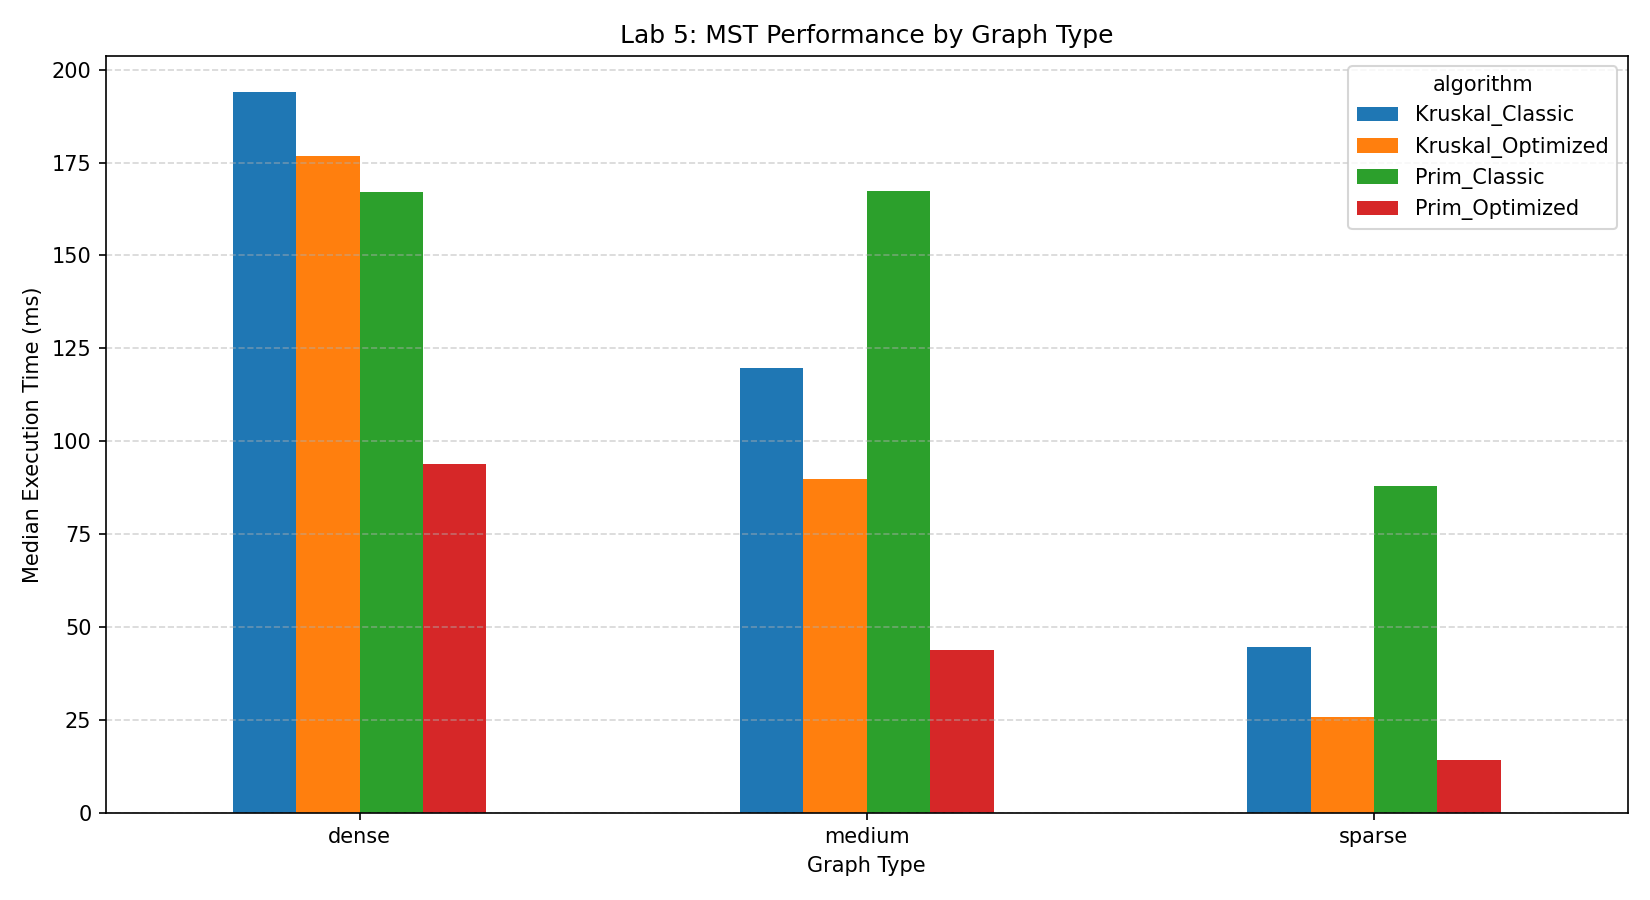
\includegraphics[width=0.88\textwidth]{../../Lab5/plots/mst_by_graph_type.png}
    \caption{MST performance by graph type}
    \label{fig:lab5-type}
\end{figure}

As Figure~\ref{fig:lab5-type} shows, density affects all four variants --- more edges means more work for every implementation.

\subsubsection{Conclusion}

Kruskal remains a strong greedy solution for MST construction, especially when combined with an efficient union-find structure. On sparse graphs the optimized variant showed a clear benefit: at 700 sparse nodes it required \(227.1\) ms against the classic's \(362.7\) ms, a speedup of \(1.6\times\). On dense graphs the advantage was smaller because the large edge list makes the sorting step dominant for both variants: at 700 dense nodes the optimized required \(546.0\) ms against the classic's \(589.3\) ms. In both cases the optimized variant also consumed less memory, owing to the compact union-find arrays compared with the set-of-sets representation of the classic implementation.

\tocsubsection{Comparative Analysis}

Both algorithms produced the same MST weight on every test case, confirming their correctness. Where they differ is in speed, memory, and how sensitive they are to graph density.

Prim optimized was the fastest variant overall, averaging a \(4.47\times\) speedup over Prim classic. The classic variant came last on every input: its \(O(V)\) linear scan costs the same regardless of how many edges are present, which wastes time on sparse graphs. Kruskal optimized was consistently faster than Kruskal classic, with the largest difference on sparse graphs where sorting is cheap and the union-find savings dominate.

Memory is where the two algorithms differ most clearly. Figure~\ref{fig:lab5-mem} shows peak consumption across all tested sizes. Prim's heap enqueues all incident edges of each newly added vertex, and on dense graphs this accumulates fast --- \(7302\) KB at 700 dense nodes. Kruskal's union-find stores only two arrays of length \(V\), so its footprint barely changes with edge count: \(1440\) KB at the same point.

\begin{figure}[H]
    \centering
    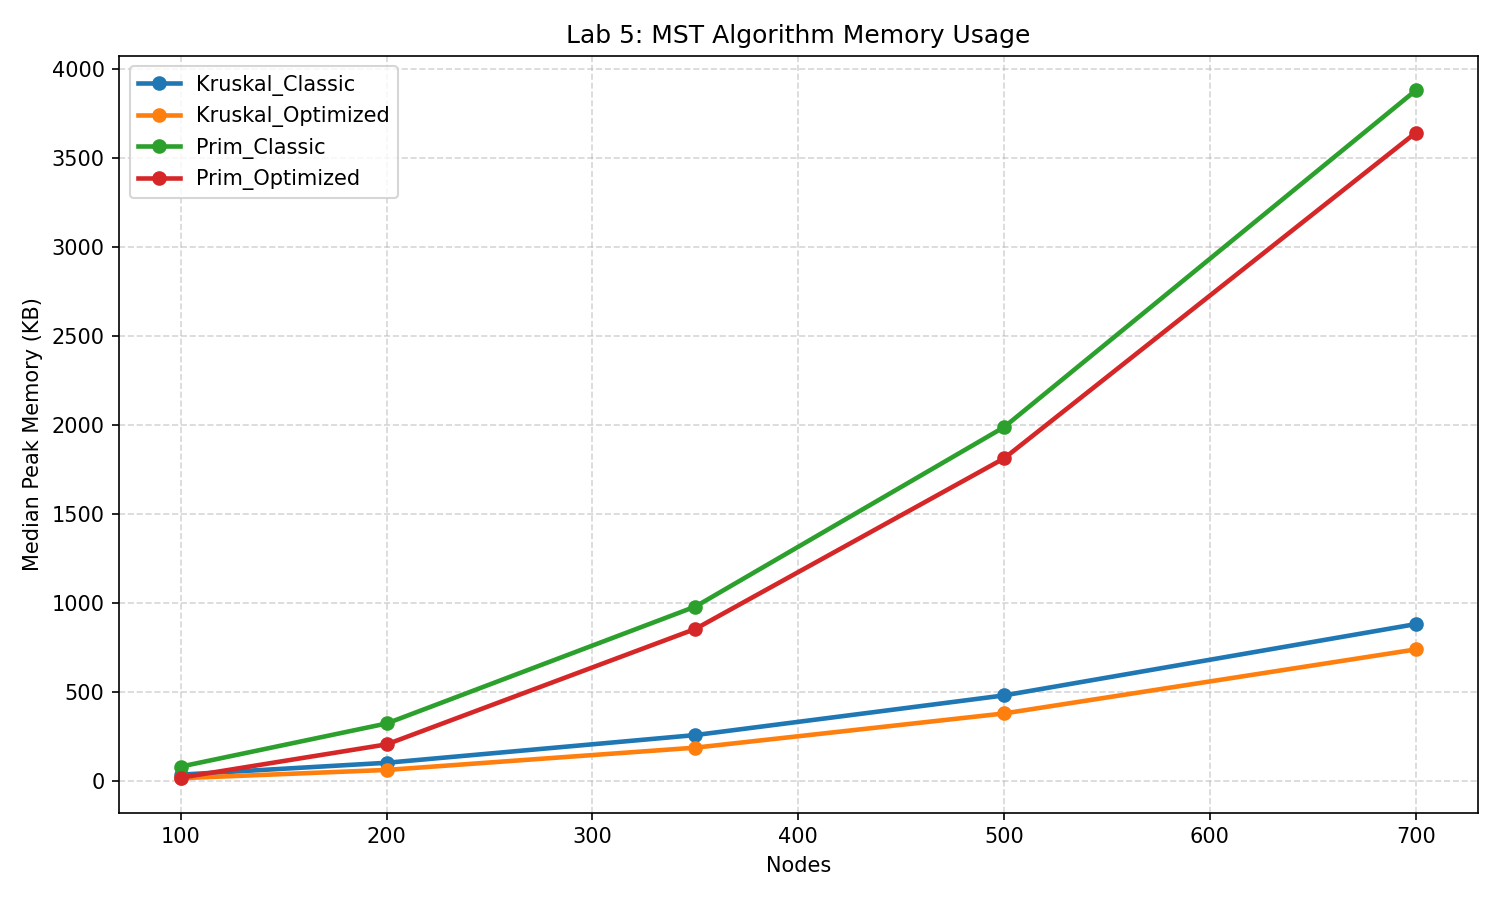
\includegraphics[width=0.88\textwidth]{../../Lab5/plots/mst_memory.png}
    \caption{Memory usage of MST algorithms across all graph sizes}
    \label{fig:lab5-mem}
\end{figure}

Figure~\ref{fig:lab5-mem-type} breaks memory usage down by density. Prim's consumption rises sharply from sparse to dense; Kruskal's stays nearly flat because the union-find size depends only on vertex count. In a memory-limited setting, Kruskal with union-find is the safer choice even when Prim optimized would be faster.

\begin{figure}[H]
    \centering
    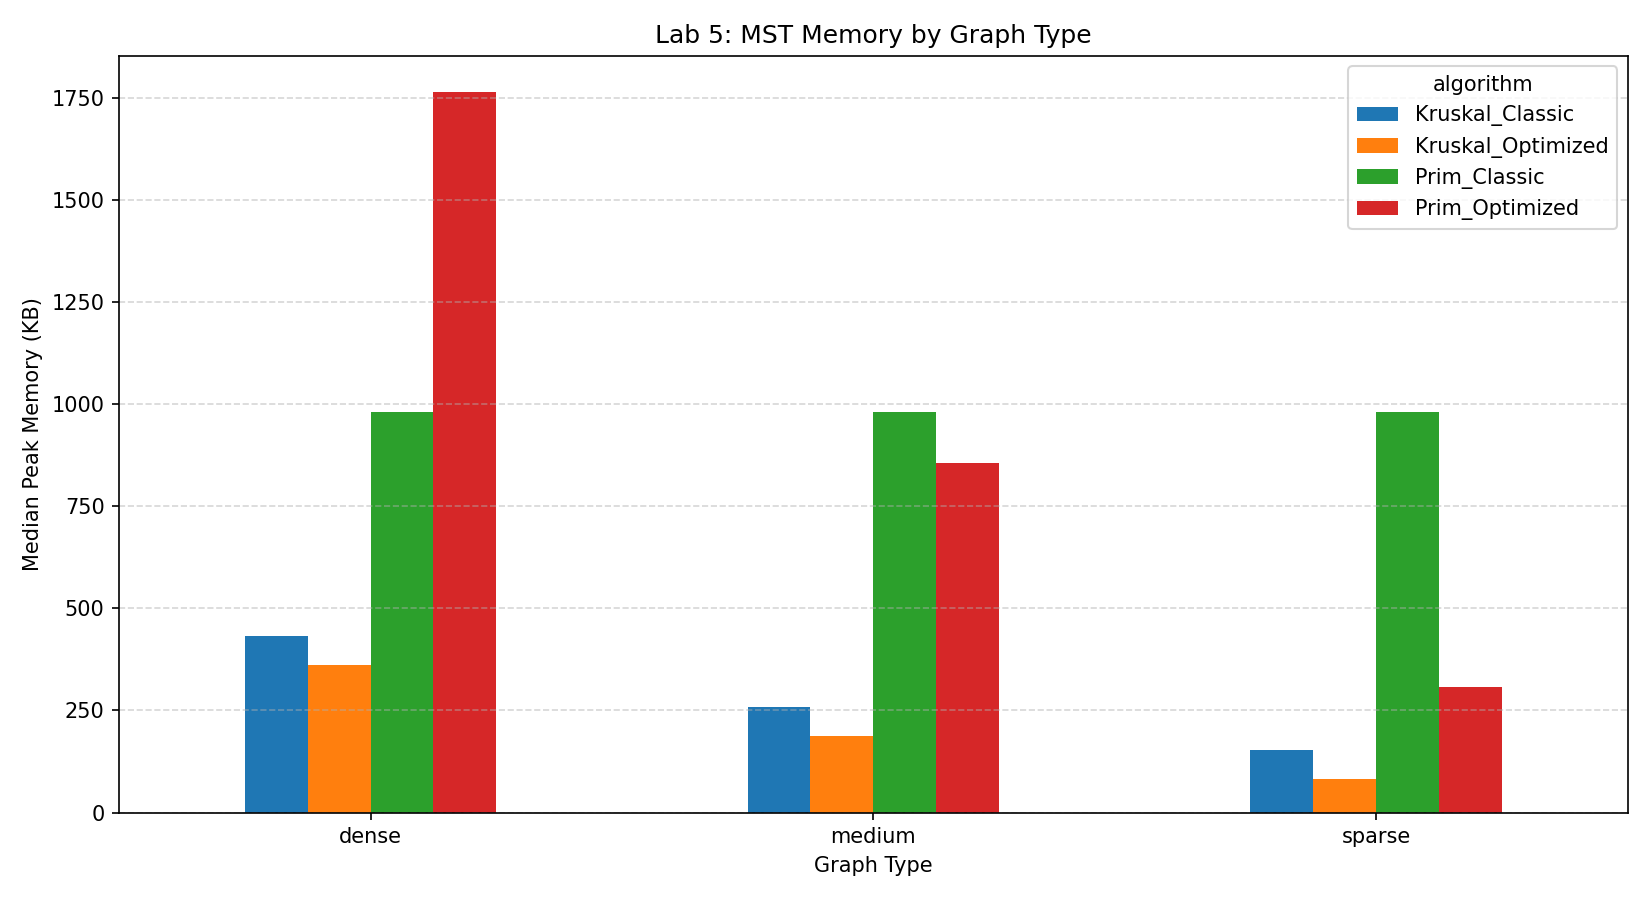
\includegraphics[width=0.88\textwidth]{../../Lab5/plots/mst_memory_by_graph_type.png}
    \caption{Memory usage of MST algorithms by graph type}
    \label{fig:lab5-mem-type}
\end{figure}

\reportunnumberedsection{CONCLUSION}
Both algorithms slowed down noticeably on denser and larger graphs, but the optimized data structures made a significant difference in both cases. Prim optimized was the overall winner, averaging a \(4.47\times\) speedup over Prim classic across the full benchmark.

Among the tested variants, Prim classic performed worst on all inputs because its \(O(V^2)\) linear scan is equally expensive regardless of edge density. The optimized Kruskal implementation improved on the classic Kruskal by \(1.6\times\) on sparse graphs but offered only modest gains on dense graphs, where the dominant cost is sorting the large edge list. Prim optimized was the fastest on both sparse and dense graphs, but at the cost of substantially higher memory usage on dense inputs.

The memory difference at 700 dense nodes --- \(7302\) KB for Prim optimized versus \(1440\) KB for Kruskal optimized --- makes the practical choice straightforward: if memory is not a concern, Prim optimized is faster; if it is, Kruskal with union-find is the safer option. Either way, the optimized implementations should be preferred over the classic ones at all tested density levels.

\reportreferences{
\bibitem{gfg-greedy}
GeeksforGeeks. \textit{Greedy Algorithms} [online]. [cited 07.05.2026]. Available: \url{https://www.geeksforgeeks.org/greedy-algorithms/}.

\bibitem{tp-greedy}
TutorialsPoint. \textit{Greedy Algorithms} [online]. [cited 07.05.2026]. Available: \url{https://www.tutorialspoint.com/data_structures_algorithms/greedy_algorithms.htm}.

\bibitem{scaler}
Scaler. \textit{Prim's and Kruskal's Algorithm} [online]. [cited 07.05.2026]. Available: \url{https://www.scaler.com/topics/prims-and-kruskal-algorithm/}.

\bibitem{repo}
Ple\c{s}u D. \textit{aa-course-repo, Lab 5 source folder} [online]. GitHub, 2026. [cited 07.05.2026]. Available: \url{https://github.com/Prince-of-Nothing/aa-course-repo/tree/main/Lab5}.
}

\end{document}
